\FILE{usecase/hvac.tex}
\subsection{Use Case: HVAC Recommendation}

\paragraph*{Background.}
The heat ventilation and air conditioning (HVAC) systems regulate the temperature in houses and buildings. 
The desired temperature can be predetermined by a technician or controlled by the user. The chosen setpoint 
is automatically sent to the HVAC, so it will start to work to meet the desired temperature in the house or 
building. However, this way of HVAC control only considers user preference as a criterion. But, to improve the 
HVAC efficiency over time, other inputs can enrich the decision-making. Those inputs are weather forecast, utility prices, 
past user preferences, period of the day, etc. Once we have this list of inputs, we develop an algorithm that can calculate 
the optimal schedule of HVAC concerning user comfort level preferences. In this way, the technician or homeowner does not 
need to change the setpoint constantly. Still, the algorithm will make the right decision within the desired user comfort 
level while reducing energy consumption and cost. The algorithm deployment is on the cloud as a service, and every time it makes a new 
setpoint decision, the command is sent to the local thermostat (see Figure \ref{fig:hvac_general}). Various service 
frequencies were used to establish the proper pipeline for this application use case. This work aims to analyze the scalability 
and adaptability of such service scenarios and identify best practices that promote reusable implementations to support aspects of 
similar use cases addressed by them.

\paragraph*{System model.}
User comfort level is defined as the allowed temperature range in the house, which is dictated by user’s personal preferences; the range can remain constant during the entire 24 hour cycle, or it can vary based on the time of the day or the day of the week (e.g. a some what higher temperature may be allowed when the occupants will be at work and away from the home). Since the temperature in the house is affected by the outdoor temperature our goal is to keep the internal temperature within the user comfort level range $Comfort = [Tmin, Tmax]$. 
Energy prices fluctuate through out the day, driven by market dynamics. We describe the pricing function as a sequence of values $Price = {P1, P2, . . . , Pm}$ where $Pi$ corresponds to the price at time slot $i$. At each time slot, the service provider determines the electricity price and charges the customer at the given rate. We determine the user cost based on the price and energy consumption during the time slot. At time $tk-1$, we observe the set of all variables of the system which includes information about the outdoor temperature, the indoor temperature, and the pricing. Based on all this information, the  algorithm makes a dynamic decision to set the HVAC set point. This represents the HVAC state in the next time-interval $tk$. After executing the HVAC action, we observe the system during time step $tk$. These steps are executed in periodic intervals, as presented in Figure \ref{fig:} and the set point recommendation process require advanced machine learning algorithm (e.g, reinforcement learning) \cite{kotevska2020rl}. Accurate recommendations can save energy and reduce cost. We organized this functionality in three parts Environmental Forecasting (EF), Learning from the past, (LP), and Set-Point Recommendation (SPR). EF calculates weather temperature and price predictions. LP learns from the behavior in the past. SPR model calculates next set-point based on past experience and EF predictions. Figure \ref{fig:hvac1_flowchart} shows the general modeling system flow chat.

\begin{figure}[htb]
\centering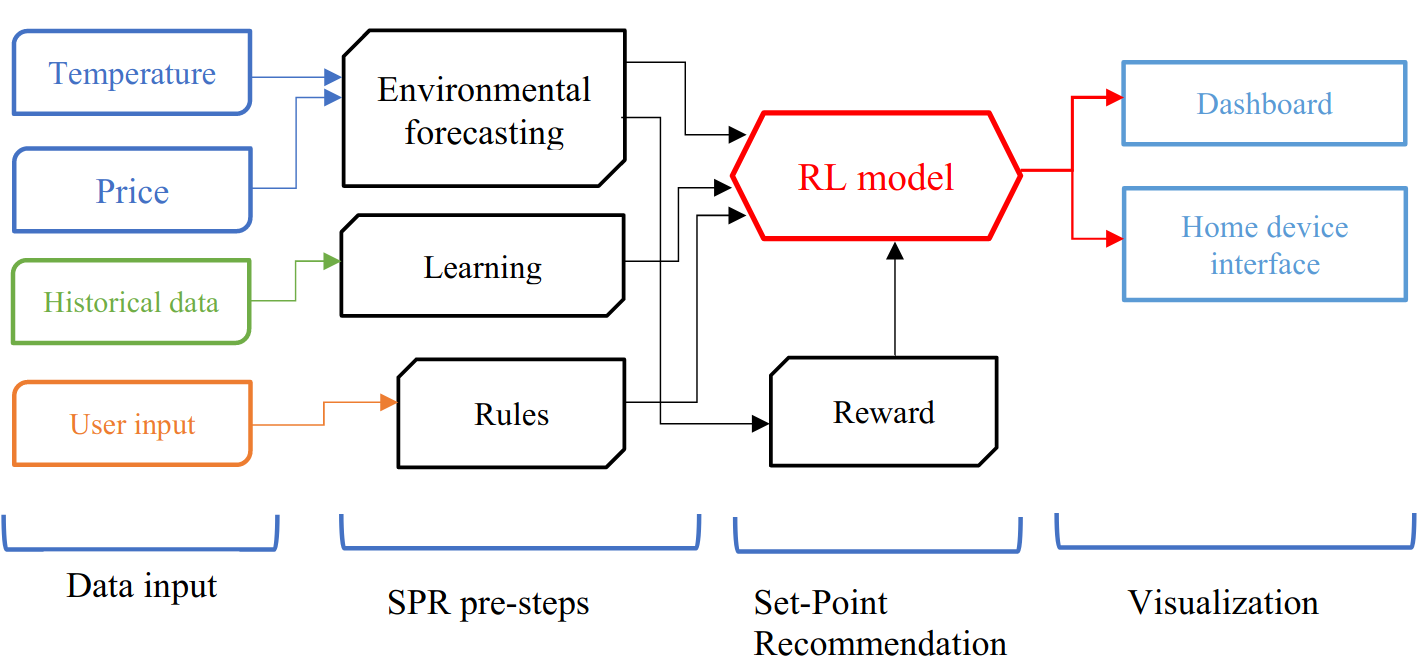
\includegraphics[width=1.0\columnwidth]{usecase/hvac.png}
\label{fig:hvac1_flowchart}
\caption{HVAC general modeling system flow chat.}
\end{figure}


\paragraph*{Functionalities and Activities} (based on Big Data Application Provider of NBDIF Ref. Architecture).

In this case study, we only focus on three main functionalities, namely EF, LP and SPR, and their activities. Figure \ref{fig:hvac2_func_diagram} shows the cross-functional diagram for their actions.



\begin{figure}[htb]
\centering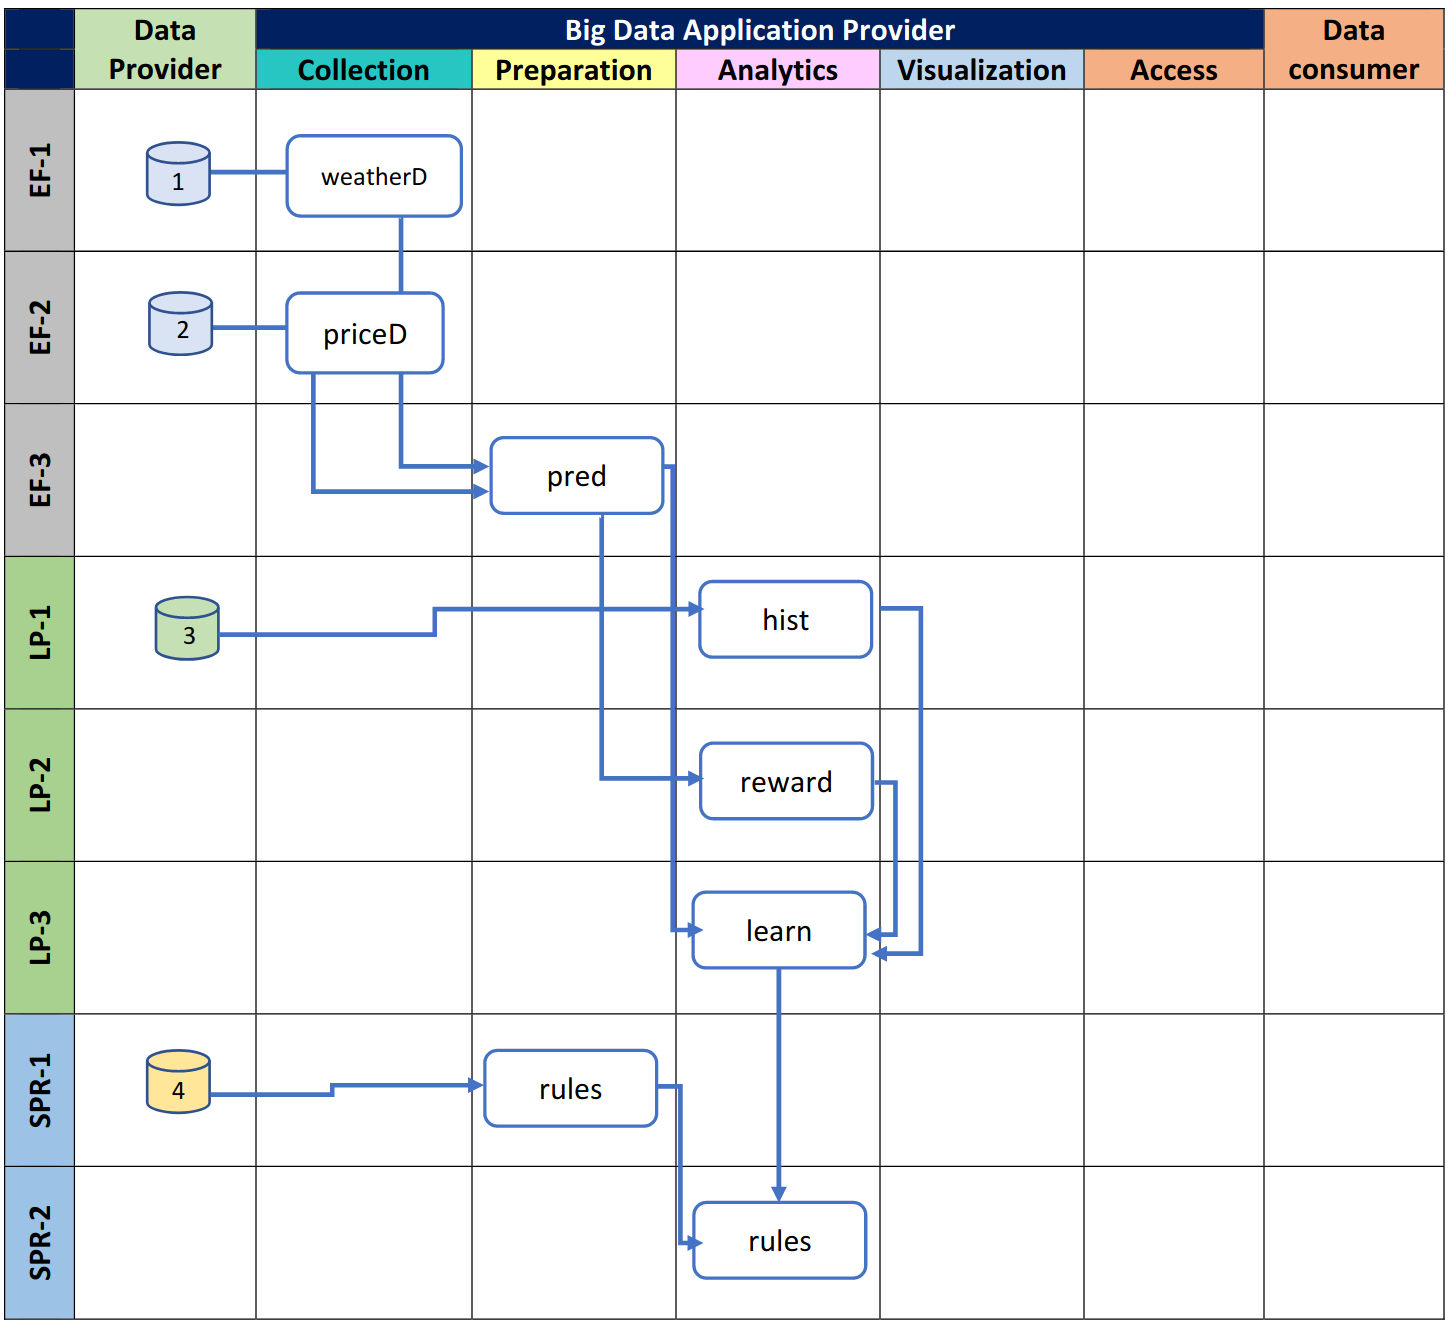
\includegraphics[width=1.0\columnwidth]{usecase/hvac-2.png}
\label{fig:hvac2_func_diagram}
\caption{Cross-Functional Diagram HVAC Recommendation.}
\end{figure}


EF Activities:

\begin{enumerate}
\item weatherD -- Collects current weather temperature and predicted temperature for timestamp X.
\item priceD -- Collects current electricity price and predicted price for timestamp X.
\item pred -- Extract needed data fields and packs it into an intermediate file format. Input data from the output of weatherD and priceD.
\end{enumerate}


LP Activities:

\begin{enumerate}
\item hist -- Prepares history data points and creates initial condition weights.
\item reward -- Generates reward based on the current weatherD and priceD.
\item learn -- Collects data from current weatherD, priced, reward.
\end{enumerate}

SPR Activities:

\begin{enumerate}
\item rules -- Creates rules based on user preferences and conversion preferences.
\item rlmodel --  Interpolates the output from learn, rules and generates set point recommendation
\end{enumerate}

\paragraph*{Algorithm}

\TODO{No datasets provided.}


